\tikzset{every picture/.style={line width=0.75pt}} %set default line width to 0.75pt        

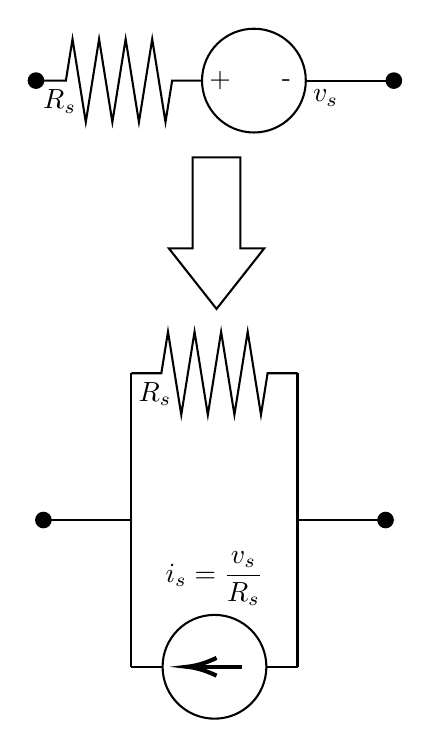
\begin{tikzpicture}[x=0.75pt,y=0.75pt,yscale=-1,xscale=1]
%uncomment if require: \path (0,420); %set diagram left start at 0, and has height of 420

%Shape: Resistor [id:dp2595676349306193] 
\draw   (201,78) -- (215.4,78) -- (218.6,58) -- (225,98) -- (231.4,58) -- (237.8,98) -- (244.2,58) -- (250.6,98) -- (257,58) -- (263.4,98) -- (266.6,78) -- (281,78) ;
%Shape: Circle [id:dp4726702298609462] 
\draw   (281,78) .. controls (281,64.19) and (292.19,53) .. (306,53) .. controls (319.81,53) and (331,64.19) .. (331,78) .. controls (331,91.81) and (319.81,103) .. (306,103) .. controls (292.19,103) and (281,91.81) .. (281,78) -- cycle ;
%Down Arrow [id:dp4867236113743594] 
\draw   (265,158.8) -- (276.5,158.8) -- (276.5,115) -- (299.5,115) -- (299.5,158.8) -- (311,158.8) -- (288,188) -- cycle ;
%Shape: Circle [id:dp48521310032792564] 
\draw   (262,360.42) .. controls (262,346.61) and (273.19,335.42) .. (287,335.42) .. controls (300.81,335.42) and (312,346.61) .. (312,360.42) .. controls (312,374.23) and (300.81,385.42) .. (287,385.42) .. controls (273.19,385.42) and (262,374.23) .. (262,360.42) -- cycle ;
%Shape: Resistor [id:dp3495898000470645] 
\draw   (247,219) -- (261.4,219) -- (264.6,199) -- (271,239) -- (277.4,199) -- (283.8,239) -- (290.2,199) -- (296.6,239) -- (303,199) -- (309.4,239) -- (312.6,219) -- (327,219) ;
%Straight Lines [id:da9040938616421672] 
\draw    (247,219) -- (247,360.42) ;
%Straight Lines [id:da4086292990449345] 
\draw    (327,219) -- (327,360.42) ;
%Straight Lines [id:da5862555045777795] 
\draw    (247,360.42) -- (262,360.42) ;
%Straight Lines [id:da15193750488345903] 
\draw    (312,360.42) -- (327,360.42) ;
%Straight Lines [id:da15177579242535977] 
\draw [line width=1.5]    (300.21,360.42) -- (276.79,360.42) ;
\draw [shift={(273.79,360.42)}, rotate = 360] [color={rgb, 255:red, 0; green, 0; blue, 0 }  ][line width=1.5]    (14.21,-4.28) .. controls (9.04,-1.82) and (4.3,-0.39) .. (0,0) .. controls (4.3,0.39) and (9.04,1.82) .. (14.21,4.28)   ;
%Straight Lines [id:da8073486658814548] 
\draw    (247,289.71) -- (204.58,289.71) ;
%Straight Lines [id:da22200817290111585] 
\draw    (369.42,289.71) -- (327,289.71) ;
%Straight Lines [id:da058000108714057586] 
\draw    (373.42,78) -- (331,78) ;
%Shape: Circle [id:dp5370808686044426] 
\draw  [fill={rgb, 255:red, 0; green, 0; blue, 0 }  ,fill opacity=1 ] (369.92,78) .. controls (369.92,76.07) and (371.49,74.5) .. (373.42,74.5) .. controls (375.35,74.5) and (376.92,76.07) .. (376.92,78) .. controls (376.92,79.93) and (375.35,81.5) .. (373.42,81.5) .. controls (371.49,81.5) and (369.92,79.93) .. (369.92,78) -- cycle ;
%Shape: Circle [id:dp007409916066804634] 
\draw  [fill={rgb, 255:red, 0; green, 0; blue, 0 }  ,fill opacity=1 ] (197.5,78) .. controls (197.5,76.07) and (199.07,74.5) .. (201,74.5) .. controls (202.93,74.5) and (204.5,76.07) .. (204.5,78) .. controls (204.5,79.93) and (202.93,81.5) .. (201,81.5) .. controls (199.07,81.5) and (197.5,79.93) .. (197.5,78) -- cycle ;
%Shape: Circle [id:dp3406177813870317] 
\draw  [fill={rgb, 255:red, 0; green, 0; blue, 0 }  ,fill opacity=1 ] (365.92,289.71) .. controls (365.92,287.78) and (367.49,286.21) .. (369.42,286.21) .. controls (371.35,286.21) and (372.92,287.78) .. (372.92,289.71) .. controls (372.92,291.64) and (371.35,293.21) .. (369.42,293.21) .. controls (367.49,293.21) and (365.92,291.64) .. (365.92,289.71) -- cycle ;
%Shape: Circle [id:dp3296743674365008] 
\draw  [fill={rgb, 255:red, 0; green, 0; blue, 0 }  ,fill opacity=1 ] (201.08,289.71) .. controls (201.08,287.78) and (202.65,286.21) .. (204.58,286.21) .. controls (206.51,286.21) and (208.08,287.78) .. (208.08,289.71) .. controls (208.08,291.64) and (206.51,293.21) .. (204.58,293.21) .. controls (202.65,293.21) and (201.08,291.64) .. (201.08,289.71) -- cycle ;

% Text Node
\draw (203,81) node [anchor=north west][inner sep=0.75pt]   [align=left] {$\displaystyle R_{s}$};
% Text Node
\draw (333,81) node [anchor=north west][inner sep=0.75pt]   [align=left] {$\displaystyle v_{s}$};
% Text Node
\draw (283,78) node [anchor=west] [inner sep=0.75pt]   [align=left] {+};
% Text Node
\draw (329,78) node [anchor=east] [inner sep=0.75pt]   [align=left] {\begin{minipage}[lt]{8.67pt}\setlength\topsep{0pt}
\begin{center}
\mbox{-}
\end{center}

\end{minipage}};
% Text Node
\draw (249,222) node [anchor=north west][inner sep=0.75pt]   [align=left] {$\displaystyle R_{s}$};
% Text Node
\draw (287,332.42) node [anchor=south] [inner sep=0.75pt]   [align=left] {$\displaystyle i_{s} =\frac{v_{s}}{R_{s}}$};


\end{tikzpicture}
